\chapter{The Generic Model Instance Type Test Suite}
\label{chapter:modelInstanceTestSuite}

\begin{flushright}
\textit{Chapter written by Claas Wilke}
\end{flushright}

To test the adaptation of a model instance type to Dresden OCL, the toolkit
provides a generic test suite that can be simply instantiated by each adapted 
model instance type. This chapter shortly presents, how the generic model
instance type test suite can be instantiated to test an adapted model 
instance type.



\section{The Test Suite Plug-in}

The generic model instance type test suite is located in the plug-in
\code{org.dresdenocl\linebreak[0].pi\-vot\linebreak[0].mo\-del\-in\-stance\-type\linebreak[0].test}.
The test suite provides a set of JUnit tests, that check the functionality of
all operations that must be adapted by every model instance type that
shall be supported for Dresden OCL. The adaptation of a model instance type
to Dresden OCL is explained in Chapter~\ref{chapter:modelInstanceTypeAdaptation}.  
The test suite contains about 100 JUnit tests.

To instantiate the generic test suite for a newly adapted model instance type,
only two resources must be provided: (1) a model instance of the newly adapted 
model instance type that contains instances of a set of model types defined in a
special test model, and (2) a Java class that instantiates the test suite with 
the model instance. During test execution, the generic test suite uses the
provided model instance to test the model instance type (cf. 
Figure~\ref{pic:modelinstancetestsuite:genericTestSuite}). Both, the model
instance and the Java class are shortly presented in the following sections.

\begin{figure}[!t]
	\centering
		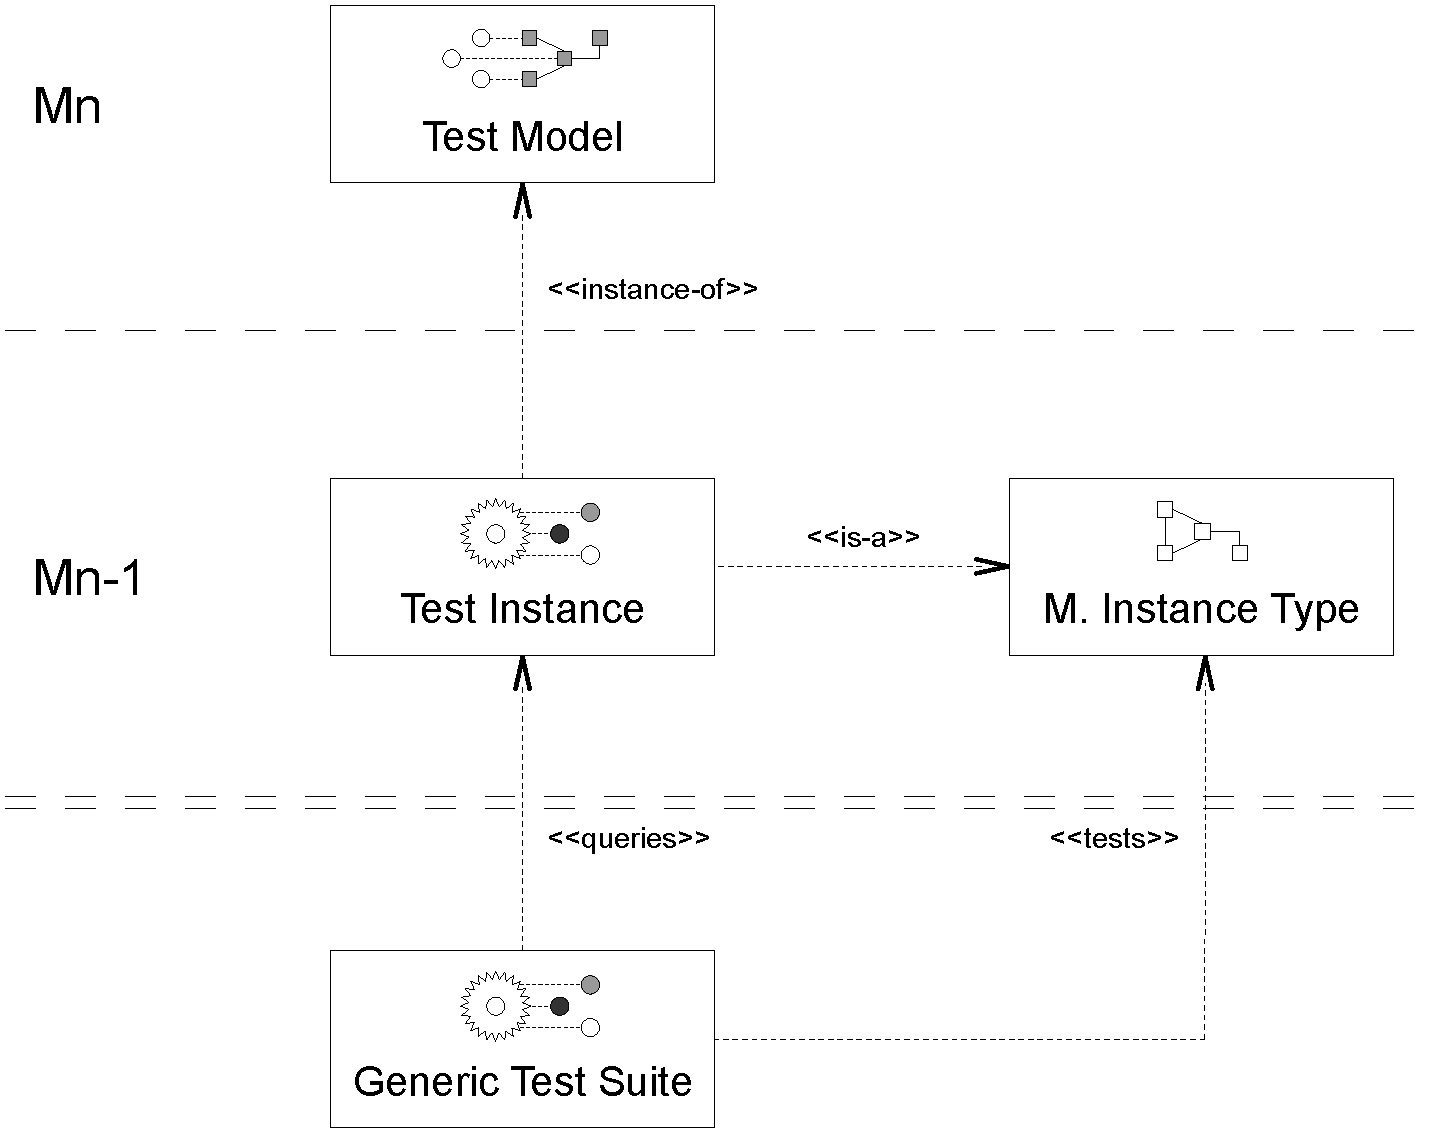
\includegraphics[width=0.80\textwidth]{figures/modelinstancetestsuite/genericTestSuite.pdf}
	\label{pic:modelinstancetestsuite:genericTestSuite}
	\caption{The Generic model instance type Test Suite in respect to the Generic
	Three Layer Ar\-chi\-tec\-ture (as presented in Section~\ref{architecture:genericLayers}).}
\end{figure}



\section{The required Model Instance to test a Model Instance Type}

The Figures~\ref{pic:modelinstancetestsuite:testModel1} 
and~\ref{pic:modelinstancetestsuite:testModel2} show the test model of which a
model instance must be provided. At a first sight, the model seems to be very 
complex. In the following, all types and relations of the test model are
explained shortly. Because a detailed explanation would be too large for this
document we recommend to investigate the already existing implementations of 
the test model provided with the test suite implementations for the Java and 
the \acs{EMF} Ecore model instance types (the plug-ins
\code{org.dresdenocl.modelinstancetype.java.test} and 
\code{org.dresdenocl.mo\-del\-in\-stance\-type.ecore.test}).

\begin{sidewaysfigure}[!p]
	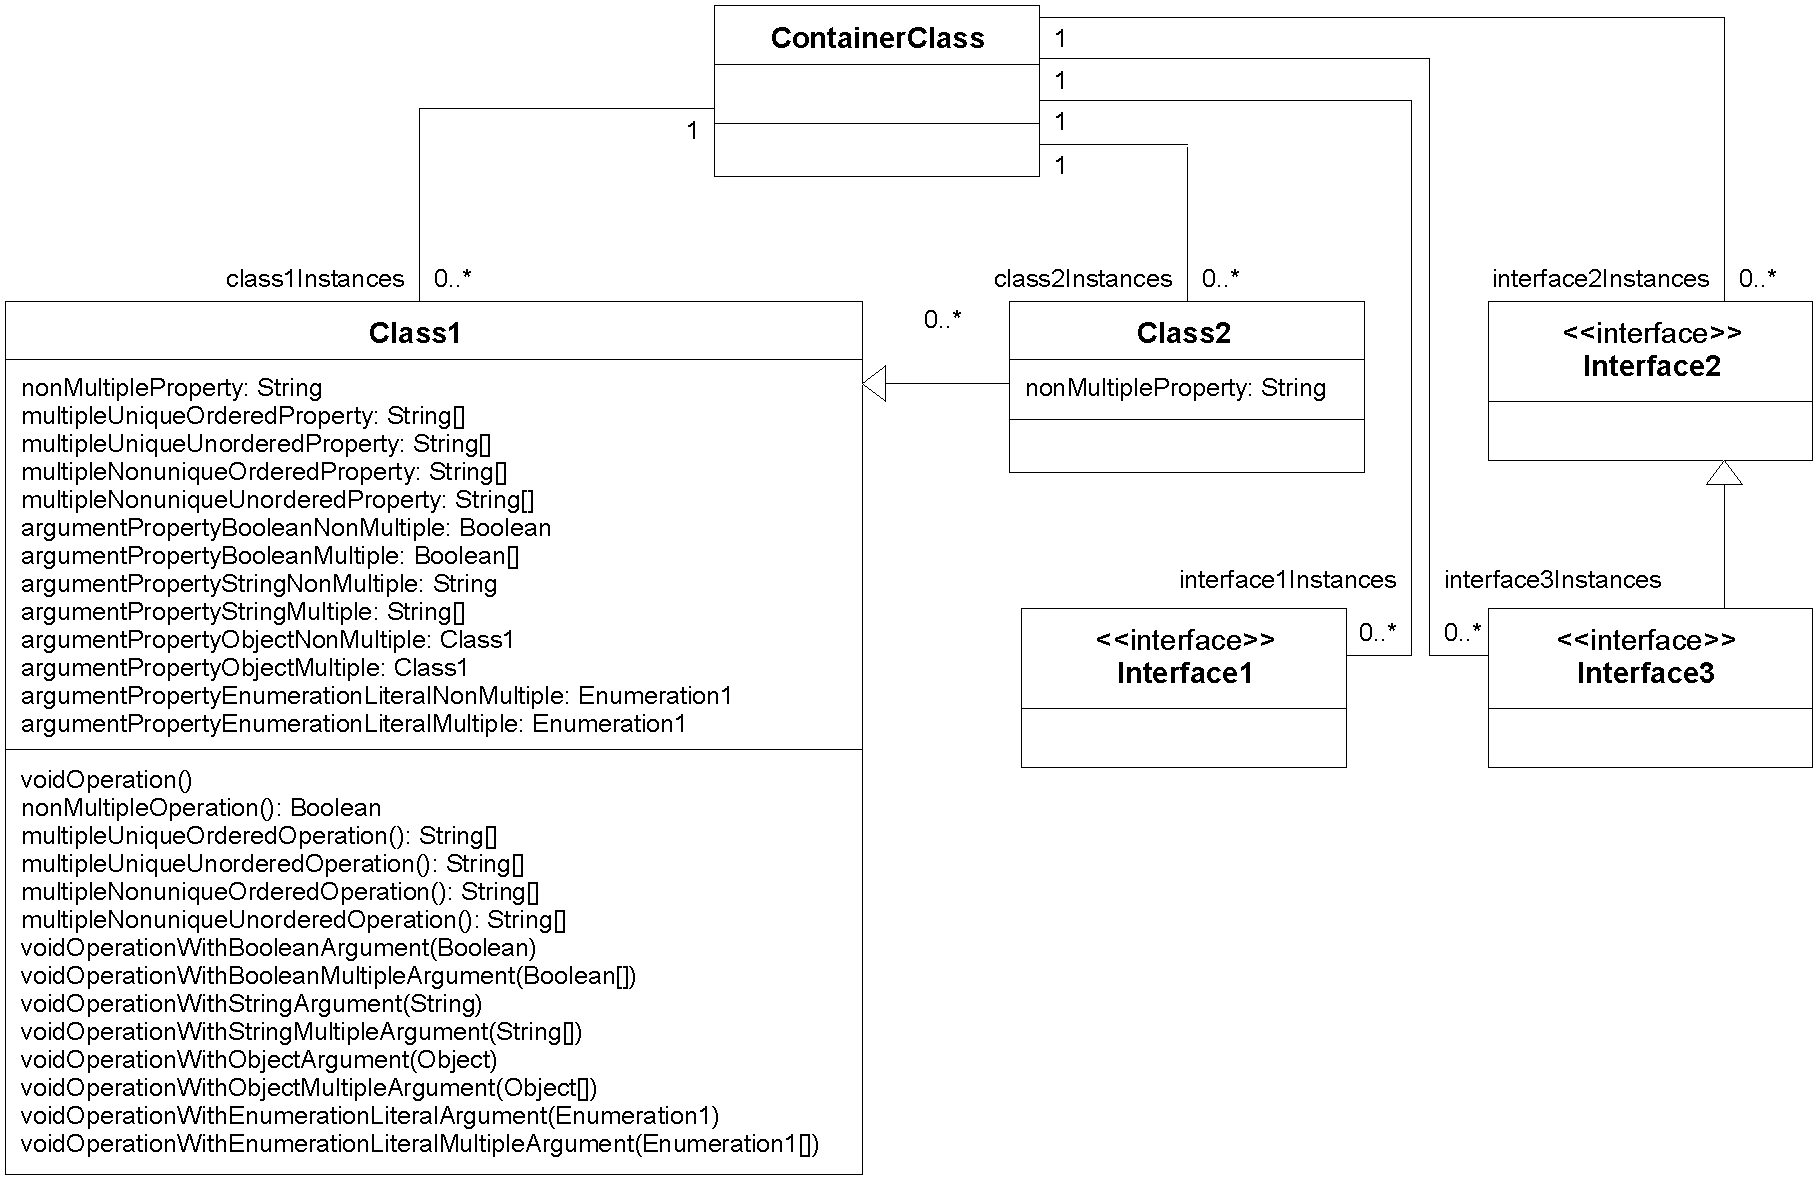
\includegraphics[width=0.9\textwidth]{figures/modelinstancetestsuite/testModel01.pdf}
	\caption{The required Test Model to test a model instance type's adaptation
	(part 1).}
	\label{pic:modelinstancetestsuite:testModel1}
\end{sidewaysfigure}

\begin{sidewaysfigure}[!p]
  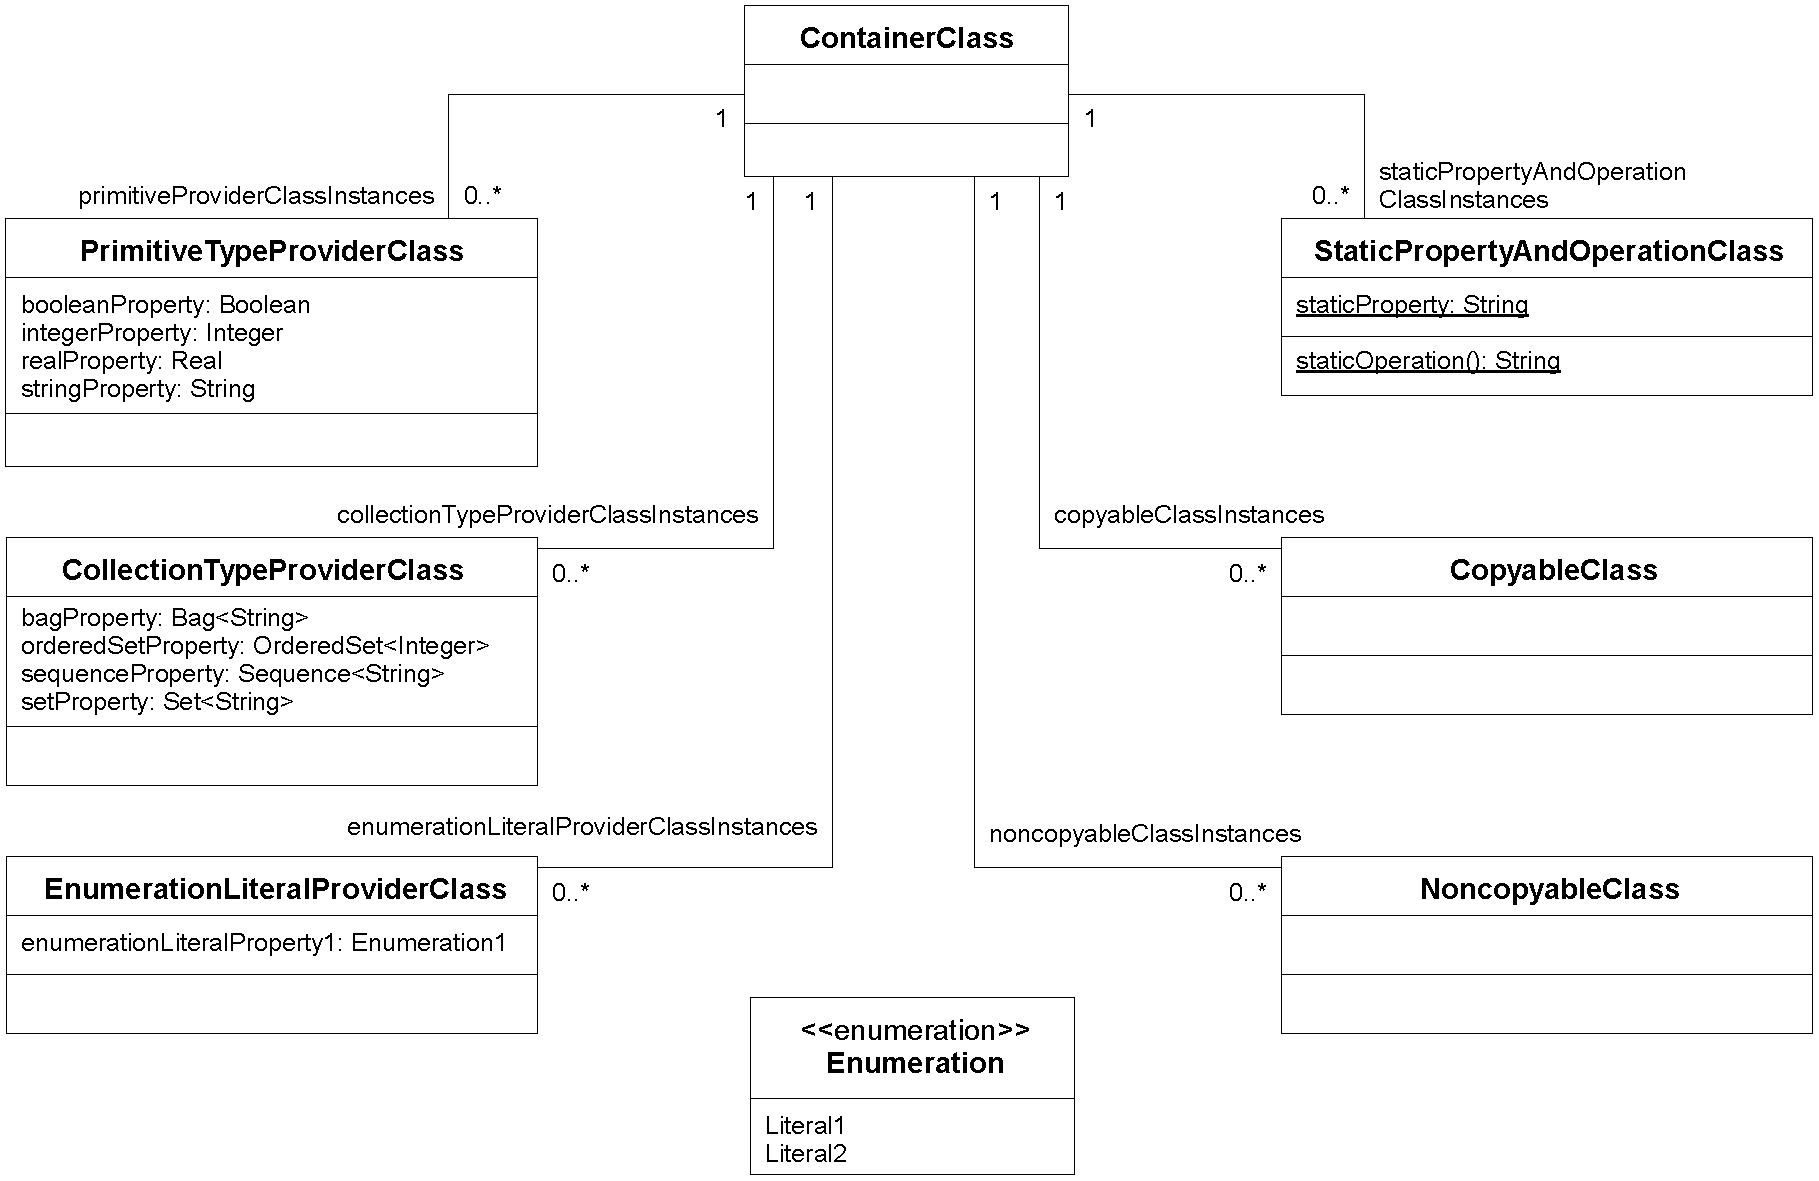
\includegraphics[width=0.9\textwidth]{figures/modelinstancetestsuite/testModel02.pdf}
	\caption{The required Test Model to test a model instance type's adaptation
	(part 2).}
	\label{pic:modelinstancetestsuite:testModel2}
\end{sidewaysfigure}


\subsection{The ContainerClass}

The \code{ContainerClass} is part of the model because in some model instance
types, each model instance must have exactly one root element that contains all 
other instance elements (e.g., EMF Ecore instances). Thus, the 
\code{ContainerClass} is responsible to manage Sets of all other classes that 
should be instantiated to test the model instance type. The
\code{ContainerClass} should be instantiated by at least one object of the 
model instance. \textbf{Please be aware that if the collections containing the 
other instance types' instances are not instantiated appropriately, the whole
test suite may fail.}


\subsection{Class1}

\code{Class1} is the major type of the model that is used to test various 
functionalities of the model instance type. It provides a set of different
properties that are used to test the right adaptation of non-multiple, 
multiple, ordered, unordered, unique and non-unique properties 
(\code{non\-Mul\-tiple\-Pro\-per\-ty}, \code{multiple...Property}). Further 
properties are required to provide default values that can be used to invoke 
the operations provided by \code{Class1} (\code{argumentProperty...}).

Besides properties, \code{Class1} provides an enormous set of operations as 
well. Some operations are responsible to test the invocation of operations  with
different result types (\code{voidOperation()}, \code{nonMultipleOperation()} 
and \code{multiple...Operation()}), others are required to test the invocation 
of operations with different argument types 
(\code{voidOperationWith...Argument()}).


\subsection{Class2}

The test model contains a second class called \code{Class2} that is used to
test casting between classes and subclasses. For the same purpose, the only 
property of the class called \code{non\-Mul\-tiple\-Pro\-per\-ty} is required. 
It is used to test the special access on parent properties in \acs{OCL} (e.g., 
by the statement \code{aClass2.oclAsType(Class1).nonMultipleProperty} which 
returns the property of \code{Class1} instead of the property of \code{Class2}).


\subsection{Interface1, Interface2 and Interface3}

The test model provides three other types called \code{Interface1}, 
\code{Interface2} and \code{Interface3}. Although the \keyword{Pivot Model}
itself does not differentiate between classes and interfaces (they are all 
handled as types internally), these three types are used to test further 
inheritance and casting relationships. The interface types should be used by 
the adapted model instance type to implement objects that extend more than one
type (multiple inheritance). If multiple inheritance is not possible for the 
adapted model instance type (not even for interfaces!) these types can be
ignored.


\subsection{PrimitiveTypeProviderClass, CollectionTypeProviderClass and 
E\-nu\-me\-ra\-tion\-Li\-te\-ral\-ProviderClass}
\label{modelInstanceTestSuite:specialTypeProviderClasses}

The classes \code{PrimitiveTypeProviderClass}, 
\code{CollectionTypeProviderClass} and 
\code{Enumeration\-Li\-teral\-ProviderClass} are responsible to provide 
instances of all model object types that shall be adapted to special-handled 
model instance objects (which are primitive types, collections (and arrays) and
enumeration literals). E.g., the \code{PrimitiveTypeProviderClass} should 
provide properties that should be handled as Booleans, Integers, Reals and 
Strings.

Because some model instance types provide different types that shall be mapped
to the same kind of type in Dresden OCL (e.g., the types \code{int} and
\code{java.lang.Integer} of Java should both be mapped to the primitive type 
\code{Integer}), these classes can provide multiple properties for the same 
type. The properties should then be numbered, ignoring the number for the first 
property and starting with the number two for the second property (e.g., if the 
\code{Pri\-mi\-tive\-Type\-Pro\-vi\-der\-Class} should provide multiple 
different \code{Integer} instances their properties should be called 
\code{integerProperty}, \code{integerProperty2}, \code{integerProperty3} and so 
on). If multiple properties for the same type are provided, the test suite must 
be informed during setup to load all the different properties (see also 
Section~\ref{modelInstanceTestSuite:setupTestSuite}).


\subsection{StaticPropertyAndOperationClass}

The \code{StaticPropertyAndOperationClass} is used to test the invocation of 
static properties and operations. Because not every model instance type supports
the invocation of static properties and operations (e.g., \acs{EMF} Ecore does 
not), these tests are based on an extra type. If the model instance type that
shall be tested does not support static features, this class could be ignored.


\subsection{Copyable- and NonCopyableClass}

\acs{OCL} supports the special operation \code{@pre} in postconditions, that can
be used in \acs{OCL} to access to values of properties' values before the 
execution of an operation that is the current context of the postcondition. To 
support this operation, the \acs{OCL} Interpreter must copy and store values of 
model instance objects.

In some model instance types it is not possible to support such a \code{copy()}
or \code{clone()} method for every single object. Thus, the test model contains 
two further types called \code{Copyable} and \code{NonCopyableClass} that should
be used to implement data structures that can be used to test the copy mechanism
during run-time explicitly.



\section{Instantiating the Generic Test Suite}
\label{modelInstanceTestSuite:setupTestSuite}

As mentioned above, to initialize the generic model instance type test suite,
only one Java class must be implemented that instantiates the test suite with
the test model instance. Listing~\ref{list:modelInstanceTestSuite:constraints01}
shows a Java class that instantiates the test suite to test the Java model
instance type.

\lstset{
  language=Java
}
\begin{lstlisting}[caption={An instantiation of the generic model instance test suite.}, captionpos=b, label=list:modelInstanceTestSuite:constraints01, float]
import org.dresdenocl.modelinstancetype.test.
       ModelInstanceTypeTestPlugin;
import org.dresdenocl.modelinstancetype.test.
       ModelInstanceTypeTestServices;
import org.dresdenocl.modelinstancetype.test.
       ModelInstanceTypeTestSuite;

@Suite.SuiteClasses(value = { ModelInstanceTypeTestSuite.class })
public class TestJavaModelInstanceType extends 
    ModelInstanceTypeTestSuite {

  /** The id of the {@link IModelInstanceTypeObject} 
    * which shall be tested. */
  private static final String MODEL_INSTANCE_ID =
    JavaModelInstanceTypePlugin.PLUGIN_ID;

  /** The path of the model which shall be tested. */
  private static final String TEST_MODELINSTANCE_PATH =
    "bin/org/dresdenocl/modelinstancetype/" +
    "java/test/modelinstance/ProviderClass.class";

  /**
   * <p>
   * Prepares the {@link ModelInstanceTypeTestSuite}.
   * </p>
   */
  @BeforeClass
  public static void setUp() {

    ModelInstanceTypeTestPlugin.prepareTest(
      JavaModelInstanceTypeTestPlugin.PLUGIN_ID, 
      TEST_MODELINSTANCE_PATH, MODEL_INSTANCE_ID);

    ModelInstanceTypeTestServices.getInstance()
      .setBooleanPropertyCounter(2);
    ModelInstanceTypeTestServices.getInstance()
      .setIntegerPropertyCounter(10);
    ModelInstanceTypeTestServices.getInstance()
      .setRealPropertyCounter(4);
    ModelInstanceTypeTestServices.getInstance()
      .setStringPropertyCounter(4);
    ModelInstanceTypeTestServices.getInstance()
      .setSequencePropertyCounter(2);
  }
}
\end{lstlisting}

Important is that the class provides a JUnit test suite (according to JUnit 4 
conventions), that contains the \code{ModelInstanceTypeTestSuite} (line 8). 
Additionally, the class only has to provide a \code{setUp()} method that can be 
used to setup the test suite before its execution (lines 22 to 45). Inside the 
\code{setUp()} method, the operation 
\code{ModelInstanceTypeTestPlugin.prepareTest(String, String, String)} must be 
invoked. The method initializes the environment of the generic test suite by 
setting three arguments:

\begin{enumerate}
	\item The \code{ID} of the plug-in that contains the test model instance used 
	  for testing (e.g.,
	  \code{tudresden\linebreak[0].ocl\-20.\linebreak[0]pivot.\linebreak[0]modelinstancetype.java.test},
	\item The location of the test model relative to the plug-in's root folder 
	  (e.g.,
	  \code{bin/org/dresdenocl\linebreak[0]/modelinstancetype/java/test/modelinstance/ProviderClass.class}),
	\item And the \code{ID} of the model instance type that shall be tested (e.g.
	  \code{org.dresdenocl\linebreak[0].pi\-vot\linebreak[0].mo\-del\-in\-stance\-type\linebreak[0].java}.
\end{enumerate}

Additionally, the method can set different counters that can be used to inform
the test suite that more than one implementation of a primitive or collection
type is provided in their provider class (lines 43 to 43, see also 
Section~\ref{modelInstanceTestSuite:specialTypeProviderClasses}).

Afterwards, the implemented Java class can be executed as a \eclipse{JUnit 
Plug-in Test} in Eclipse. The test suite should then inform you (by failed test 
cases) which parts of your model instance type adaptation are wrong implemented
or missing. Warnings caused by missing parts of the test model instance--that 
were not implemented intentionally--can be ignored.


\section{Summary}

This chapter shortly introduced into the generic model instance type test suite
of Dresden OCL. For further details of the test suite investigate the test suite
plug-in
\code{org.dresdenocl\linebreak[0].pi\-vot\linebreak[0].modelinstancetype.test} 
or the existing test suite instantiations in the plug-ins
\code{tu\-dres\-den\linebreak[0].ocl20\linebreak[0].pi\-vot\linebreak[0].modelinstancetype.java.test},
and \code{tudresden\linebreak[0].ocl\-20.pivot.mo\-del\-in\-stance\-type\linebreak[0].ecore.test}.
